% Roll no 58, Sinadin Zidan
\textbf{\textcolor{LightMagenta}{ What are the different methods for measuring classifier performance? (May 2019) \hfill 4 marks}} \\[5pt]

For classification, especially for two-class problems, a variety of measures has been proposed \\


\begin{tabular}{|p{2cm}|p{8.075cm}|}
    \hline
    & \textcolor{purple}{Predicted Class} \\
\end{tabular}\\
\begin{tabular}{|p{2cm}|p{3.1cm}|p{3.1cm}|p{1cm}|}
    \hline
     True class & Positive & Negative & Total  \\
     \hline
     Positive & tp: true positive & fn: false negative & p \\
     Negative & fp: false positive & tn: true negative & n \\
     \hline
     Total & p' & n' & N \\
    \hline
\end{tabular}

\\ \\
After we classify a data set based on a chosen learning method using positive and negative
examples, we can compare to see how many examples from test are classified correctly. There are four possible cases, as shown in table.
\begin{enumerate}
    \item {For a positive example, if the prediction is also positive, this is a \textbf{true positive (tp)}}
    \item {If our prediction is negative for a positive example, this is a \textbf{false negative (fn)}}
    \item {For a negative example, if the prediction is also negative, we have a \textbf{true negative(tn)}}
    \item {If we predict a negative example as positive it is a \textbf{false positive (fp)}.}
\end{enumerate} 

If we predict a negative example as positive it a false positive (fp).
Example consider an authentication model, users log on to their accounts by voice. A false
positive is wrongly logging on an impostor and a false negative is refusing a valid user. It is
clear that the two type of errors are not equally bad; the former is much worse\\ [0.2cm]
True positive rate, \textbf{tp-rate}, also known as \textbf{hit rate}, measures what proportion of valid users we
authenticate and false positive rate, \textbf{fp-rate}, also known as \textbf{false alarm rate}, is the proportion
of impostors we wrongly accept. \\ 
\begin{center}
\begin{tabular}{|c|c|}
    \hline
    Name & Formula \\
    \hline
    error & (f_p + f_n)/N \\
    accuracy & (t_p + t_n)/N = 1 - error \\
    \hline
    t_prate & t_p/p \\
    f_prate & f_p/n \\
    \hline
    precision & t_p/p' \\
    recall & t_p/p = t_prate \\
    \hline
    sensitivity & t_p/p = t_prate \\
    specificity & t_n/n = 1 - f_prate \\
    \hline
\end{tabular}
\end{center}
\\
\textcolor{purple}{\underline{Precision, Recall, Sensitivity, Specificity and Class Confusion Matrix}} \\
 We consider an example from information retrieval ,\\[0.2cm]
Consider there is a database of records; we make a query, for example, by using some
keywords, and a system (basically a two-class classifier) returns a number of records.\\ [0.2cm]
In the database, there are relevant records and for a query, the system may retrieve some of
them (true positives) but probably not all (false negatives); it may also wrongly retrieve records
that are not relevant (false positives).\\[0.2cm]
The set of relevant(L) and retrieved records(R) can be visualized using a Venn diagram, as
shown in figure a. \\ 

\begin{center}
    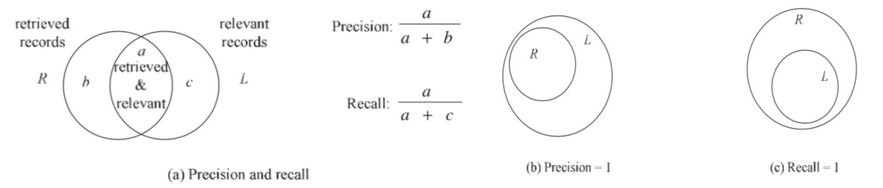
\includegraphics[width=.8\textwidth]{Images/A20_img1.png}
\end{center}

Fig (a) Definition of precision and recall using Venn diagrams. Fig b (b) Precision is 1; ie all
the retrieved records are relevant but there may be relevant ones not retrieved. Fig (c) Recall is
1; ie all the relevant records are retrieved but there may also be irrelevant records that are
retrieved. L is the set of relevant records and R is the set of Retrieved records. \\

\textcolor{purple}{\underline{Precision}} is the number of retrieved and relevant records divided by the total number of
retrieved records; if precision is 1, all the retrieved records may be relevant but there may still
be records that are relevant but not retrieved. \\

\textcolor{purple}{\underline{Recall}} is the number of retrieved relevant records divided by the total number of relevant
records; even if recall is 1, all the relevant records may be retrieved but there may also be
irrelevant records that are retrieved, as shown in figure c. \\

\textcolor{purple}{\underline{Sensitivity and specificity}} From another perspective but with the same aim, there are the
two measures of \textit{sensitivity} and \textit{specificity}. Sensitivity is the same as tp-rate and recall.
Specificity is how well we detect the negatives, which is the number of true negatives divided
by the total number of negatives; this is equal to 1 minus the false alarm rate. One can also
draw a sensitivity vs. specificity curve using different thresholds.\\

\textcolor{purple}{\underline{Class confusion matrix:}} In the case of no of classes K > 2 classes, if we are using 0/1 error, the class confusion matrix is a K × K matrix whose entry (i, j) contains the number of instances that belong to C\textsubscript{i} but are assigned to C\textsubscript{j} . Ideally, all off-diagonals should be 0, for no misclassification. The class confusion matrix allows us to pinpoint what types of misclassification occur, namely, if there are two classes that are frequently confused. Or, one can define K separate two-class problems, each one separating one class from the other K-1. \\

\begin{center}
    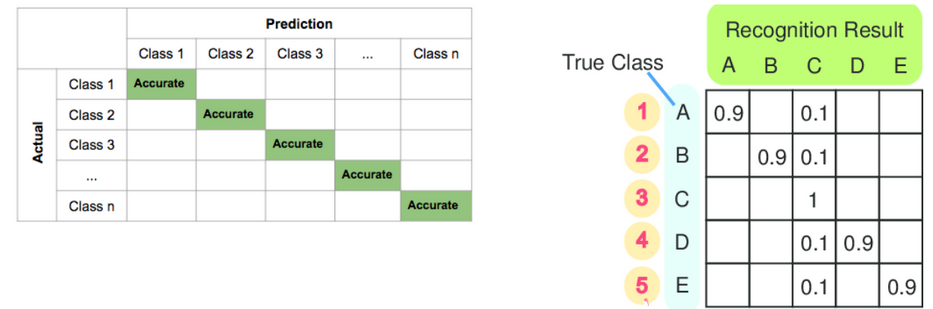
\includegraphics[width=.8\textwidth]{Images/A20_img2.png}
\end{center}

Consider the example – there are five classes (A, B, C, D, E), the diagonal shows percentage of classes that are rightly classified. Index(1, 3) shows a miss classification i.e – .1 examples from class A is classified into Class C. Similarly ((2, 3), (4, 3),(5, 3)) also shows unclassified percentage. \\ 